%!TEX root = report.tex
\section{Introduction}

\setlength{\parskip}{1em}

With the growing number of robots for a big variety of applications, it gets more and more important that a robot can autonomously detect its environment and position itself with respect to obstacles and objects of interest. 
The corresponding research area of Simultaneous Localization and Mapping (SLAM) is therefore growing exponentially. 
In addition to ever-improving algorithms, an increasing range of sensors to perceive the environment are also being adopted for SLAM applications. 

A new method for SLAM using acoustic echoes, called echo-SLAM, is being developed at the \textit{Laboratoire des communications audiovisuelles} (LCAV) \cite{Miranda}. The inspiration for this method comes from blind people who are able to navigate in unknown environments by detecting the echoes of sound signals they emit. The idea of the algorithm is to measure the so-called ``room impulse response'' to relate the geometry of the room to the intensity of the recorded echoes from different walls. 

Determining the actual geometry of the room requries several measurements, performed at different locations. 
For this reason, an ``acoustic robot'' has been developed that can be remotely controlled to take predetermined steps, estimate its displacement using odometry and record the room impulse response when at rest. 

The goal of this project is to provide an experimental framework for operating the robot and taking acoustic measurements. 
A main feature of the proposed framework is that the ground truth for the robot position is calculated using a visual localization technique. 
This technique uses four cameras whose positions are calculated with image- to-object-space correspondances. 
The real coordinates of any point in the camera's images can then be obtained by geometric transformations, allowing the robot to be localized in the room.
A diagram of the framework is given in Figure \ref{fig:setup}. 

Multiple analysis tools for the visual, audio and odometry results are also provided, allowing for an extensive automated evaluation of the obtained experimental results. 
Finally, the experimental framework and the analysis tools are employed in several sets of experiments and continuously improved. A comprehensive documentation of the used hardware and software is created, allowing for later use within the laboratory.  


\begin{figure}[b]
    \centering
    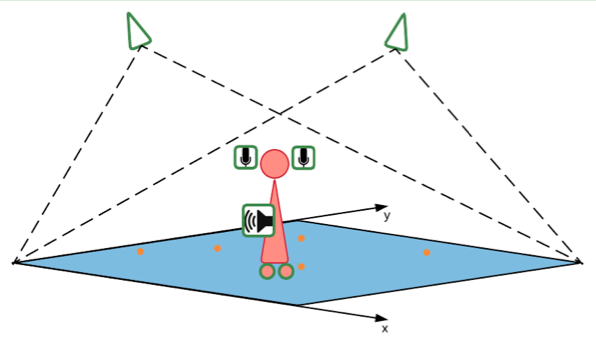
\includegraphics[width=.6\linewidth]{files/Setup.png}
    \caption{Diagram of experimental setup for Echo-}
    \label{fig:setup}
\end{figure}
